\documentclass[12pt]{article}
\usepackage[margin=0.7in]{geometry} 		% defines page margin
\usepackage{knitting} 				% defines \chart and \textknit
\usepackage{titling} 				% title page
\usepackage{graphicx,xspace, scrextend}	% defines space control stuff
\usepackage{tabularx, array, colortbl}	% defines tables
\usepackage{multicol} 				% defines columns
\usepackage{multirow} 				% defines multirows, combined cells in tables
\usepackage{framed} 				% defines boxes for notes and written directions
\usepackage[x11names]{xcolor} 		% extends color library
\pdfmapfile{+knitfont.map}

\renewcommand{\arraystretch}{2}

\newcolumntype{L}[1]{>{\leftalign\arraybackslash}p{#1}}
\newcolumntype{C}[1]{>{\centering\arraybackslash}p{#1}}

% length parameters
\setlength{\parindent}{0pt} % disables indentation for paragraphs
\setlength{\columnsep}{0.7cm} % column separation in multicol environment

% color parameters
\colorlet{framecolor}{black}
\colorlet{shadecolor}{LemonChiffon1}
\colorlet{highlight}{yellow}

% custom commands
\newcommand{\comment}[1]{} % allows for multiline comments that LaTeX will ignore

\newcommand{\vocab}[1]{\emph{\textbf{#1}}} % format for highlighting definitions of stitches, vocabulary terms
\newcommand{\rowDir}[1]{\textbf{#1:}} % indent for written instructions within paragraphs

\renewcommand{\repeat}[1]{\textbf{*[#1]*}} % format for written repeats, bold with *[ stitches ]*

\newcommand{\increase}[1]{(\emph{+#1 
	\ifnum#1=1{st}\else{sts}\fi})}
\newcommand{\decrease}[1]{(\emph{$-$#1
	\ifnum#1=1{st}\else{sts}\fi})}
\newcommand{\stitchcount}[1]{(\emph{#1 sts})}

\newcommand{\blank}{\underline{\hspace{2em}} }

% thick horizontal line
\makeatletter \newcommand{\thickhline}{
    \noalign {\ifnum 0=`}\fi \hrule height 1.5pt
    \futurelet \reserved@a \@xhline
}
\makeatother

% custom environments
\newenvironment{frnote}
    {% framed environment for pattern notes
    	\setlength{\FrameRule}{1.5pt}
    	\def\FrameCommand{\fboxrule=\FrameRule\fboxsep=\FrameSep \fcolorbox{framecolor}{shadecolor}}
    	\MakeFramed {\FrameRestore}}
    {\setlength{\FrameRule}{1pt}
	\endMakeFramed}

\newenvironment{frdirection}
    {% framed environment for written directions
	\def\FrameCommand{\fboxrule=\FrameRule\fboxsep=\FrameSep \fbox}
   	\MakeFramed {\advance\hsize-\width \FrameRestore}
    	\addmargin[1.5cm]{0pt}}
    {\endaddmargin
	\endMakeFramed}

\newenvironment{unframed}
    {% unframed environment for written directions
	\begin{addmargin}[2em]{0pt}
	\setlength{\parindent}{-2em}}
    {\vspace{1em}
	\setlength{\parindent}{0em}
	\end{addmargin}}

\title{Pops and Pins}
\author{Shanel Wu (Piper Nell)}

\begin{document}
\begin{titlingpage}

\begin{multicols}{2}
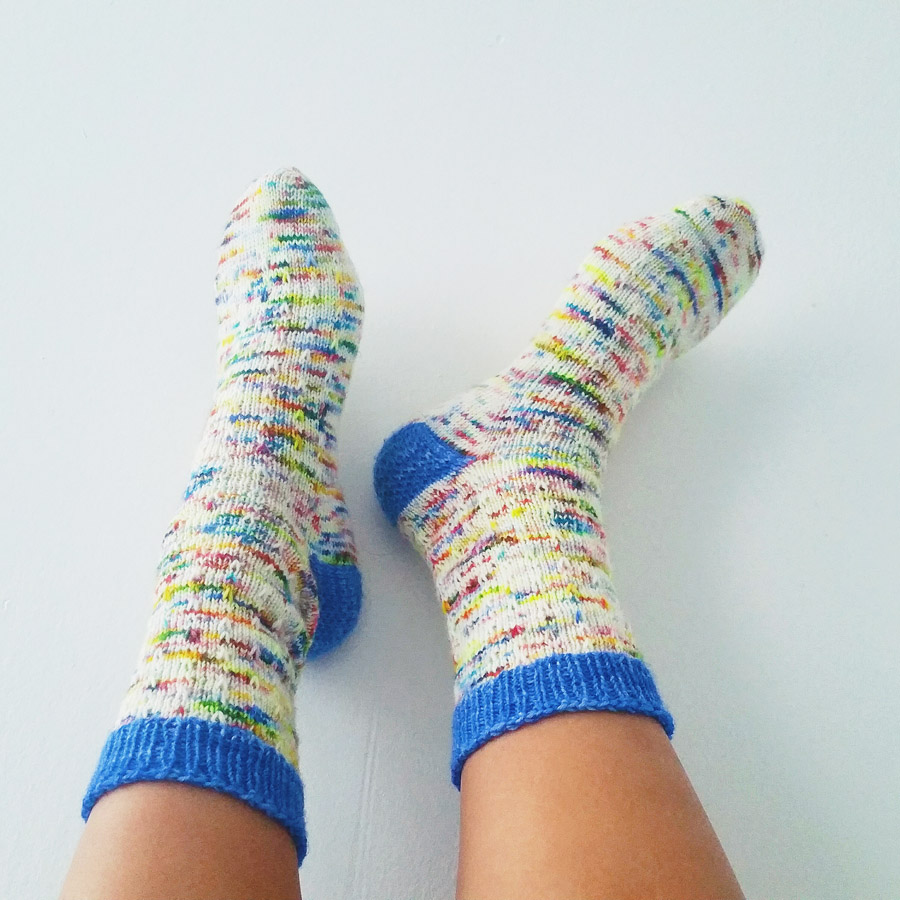
\includegraphics[height=3.5in]{feetWall.jpg}

\section*{\thetitle}
\vspace{-0.5em}
\subsubsection*{\theauthor}

Grab a skein of speckled yarn and watch the colors \emph{pop} in a slip-stitch \emph{pins} texture!

\vspace{-1em}
\subsubsection*{Materials}

\begin{itemize}
\item 100g sock yarn in MC
\item 20g sock yarn in CC (optional)
\item Your favorite sock needles
\end{itemize}

\subsubsection*{Using This Recipe}

This version of the sock pattern is not a full pattern, but a worksheet for how to use the main texture with your preferred sock techniques. It is written to be needle-agnostic, but may be biased towards Magic Loop. 

\vspace{1em}
The ``Pops and Pins" texture repeat is 8 stitches by 8 rows, so it can be used on a 48, 56, 64, or 72 (or any other multiple of 8) stitch sock. 

\vfill

\subsection*{Main Texture - ``Pops and Pins"}

\small
\begin{tabular}{| C{0.12\linewidth}  C{0.2\linewidth}  p{0.55\linewidth} | }
\thickhline \rowcolor{shadecolor} 
\textbf{Chart}	& \textbf{Written}	& \textbf{Name \& Description} \\ \thickhline
\chart{-}	& k	&  knit	\\
\chart{v}	& s1		& \textbf{slip 1} stitch purlwise with yarn in back (wyib) \\
\chart{z}	& w2k		& \textbf{wrap 2 knit:} insert needle into stitch as if to knit, wrap yarn twice and pull both loops through; produces doubled stitch \\
\chart{Y}	& s1dl		& \textbf{slip 1 drop loop:} slip doubled stitch wyib, drop second wrap \\ \hline
\end{tabular}

\normalsize

\subsection*{Chart}

\chart{
\!\overline{--------}\! \rnright
\!-v------\! \rnright
\!-Y---v--\! \rnright
\!-z------\! \rnright
\!--------\! \rnright
\!-----v--\! \rnright
\!-v---Y--\!\rnright
\!\underline{-----z--}\! \rnright
}

\small
\subsection*{Written}

\rowDir{Rnd 1} k2, \repeat{w2k, k7}, w2k, k5

\rowDir{Rnd 2} k2, \repeat{s1dl, k3, s1, k3}, s1dl, k3, s1, k1

\rowDir{Rnd 3} k2, \repeat{s1, k7}, s1, k5

\rowDir{Rnd 4} k across

\rowDir{Rnd 5} k6, \repeat{w2k, k7}, w2k, k1

\rowDir{Rnd 6} k2, s1dl, k3, \repeat{s1dl, k3, s1, k3}, s1dl, k1

\rowDir{Rnd 7} k6, \repeat{s1, k7}, s1, k1

\rowDir{Rnd 8} k across

\normalsize

\newpage
\section*{Set Up}

Choose your \vocab{sock circumference (SC)}:
\begin{center}\textbf{My socks are \blank sts around.}			\end{center}

Next, look up the number of repeats to be worked across the foot instep \vocab{(FR)} and the number of repeats to be worked around the leg \vocab{(LR)}. If FR is not a whole number -- for example, if FR is 3.5 repeats, then you must work 3 whole repeats and the first 4 sts of another repeat.

\begin{center}
\begin{tabular}{| C{0.15\linewidth} | C{0.3\linewidth} | C{0.25\linewidth} |}
\hline 
\textbf{SC}		& \textbf{FR}	& \textbf{LR} \\ \hline
48 sts			& 3 repeats			& 6 repeats \\
56 sts			& 3.5 repeats		& 7 repeats \\
64 sts			& 4 repeats			& 8 repeats \\
72 sts			& 4.5 repeats		& 9 repeats \\
$n$ sts		& $n/16$ repeats		& $n/8$ repeats \\ \hline
\end{tabular}
\end{center}

\section*{Toe Up Instructions}

\begin{enumerate}
\item \rowDir{Toe} With your preferred toe method, cast on and increase until the sock has \vocab{SC}~=~\blank sts.

\item \rowDir{Foot} Divide your stitches in half to designate ``sole sts" and ``instep sts". Work \vocab{FR}~=~\blank repeats of the ``Pops and Pins" texture across the instep sts. K across sole sts (stockinette st). Stop when foot is the desired length, and make a note of which repeat round you last worked: Rnd \blank.

\item \rowDir{Heel} Your ``sole sts" will now become your ``heel sts". Work your preferred heel method on the heel sts, making sure that you still have \vocab{SC} sts after the heel.

\item \rowDir{Leg} Your ``heel sts" will now become your ``back sts" while the ``instep sts" are now the ``front sts". 
\vspace{1em} \\  If you stopped in Step 2 \textbf{after working Rnd 4 or 8:} proceed to the next paragraph. If you stopped \textbf{after \emph{any other} round:} continue texture along front sts \emph{ONLY} (work back sts in stockinette) until you finish either Rnd 4 or Rnd 8, then proceed. 
\vspace{1em} \\ Work \vocab{LR}~=~\blank repeats of the ``Pops and Pins" texture across both the front and back sts of the sock, stopping after Rnd 4 or Rnd 8.

\item \rowDir{Cuff} Any rib pattern that is a 4 st or 2 st repeat will pair well with the texture. (e.g. 1x1, 2x2, 3x1) Work chosen rib pattern until cuff is the desired length, then bind off with a stretchy BO.
\end{enumerate}

\section*{Cuff Down Instructions}

Using the texture on a cuff down sock will result in inverted the V's to become ``wishbones". Because I have only used this texture on a toe up sock, use these instructions at your own risk.

\begin{enumerate}
\item \rowDir{Cuff} Cast on \vocab{SC}~=~\blank sts with a stretchy CO. Work chosen rib pattern until cuff is the desired length.
\item \rowDir{Leg} Work \vocab{LR}~=~\blank repeats of the ``Pops and Pins" texture around the leg.
\item \rowDir{Heel} Work your preferred heel method, making sure that you still have \vocab{SC} sts after the heel.
\item \rowDir{Foot} Work \vocab{FR}~=~\blank repeats of the ``Pops and Pins" texture across the instep and work sole sts in stockinette. 
\item \rowDir{Toe} Work preferred toe method and kitchener graft, if needed.
\end{enumerate}

\vfill

\newpage
\end{multicols}

\end{titlingpage}

\end{document}